
%4%%4%%4%%4%%4%%4%%4%%4%%4%%4%%4%%4%%4%%4%%4%%4%%4%%4%%4
%             Conceituação das soft skills             %
%4%%4%%4%%4%%4%%4%%4%%4%%4%%4%%4%%4%%4%%4%%4%%4%%4%%4%%4

\chapter{Conceituação das soft skills}

\label{chap:concepts}
\thispagestyle{empty} % retira numeracao da pagina, conforme as normas de apresentacao.

Neste capítulo, explicamos a importância das soft skills que escolhemos para esta pesquisa, as quais foram listadas no Capítulo \ref{chap:research}, discutindo suas aplicações na profissão do programador de software. O objetivo deste capítulo é esclarecer o significado de cada soft skill e encontrar informações suficientes para desenvolver formas de identificá-las automaticamente.

A importância de entender e identificar soft skills já foi discutida anteriormente, na Subseção \ref{subsec:ss-importance}. Focando no papel de programdor, essa relevância não deixa de ser uma realidade, pois as empresas de desenvolvimento de software precisam encontrar indíviduos qualificados para preencher os requisitos da profissão.

O conhecimento a respeito das soft skills também é necessário para o próprio programador, para que o mesmo possa entender as exigências do ambiente de trabalho em que atua e ainda reconhecer seus pontos fortes e características que precisam ser melhoradas. Adicionalmente, esse conhecimento auxilia educadores a encorajar o desenvolvimento de importantes habilidades em seus educandos.

Para melhor entender o significado de cada soft skill abordada por este trabalho, categorizamos as soft skills de acordo a proposta de Joseph et al. \cite{joseph:99} \cite{joseph:10}, que define cada habilidade como uma estratégia para gerenciamento de tarefas, gerenciamento de si próprio, gerenciamento da carreira ou gerenciamento dos outros. Esta organização foi apresentada na Subseção \ref{subsec:ss}.

Além disso, propomos um mapeamento das soft skills com os fatores de personalidade descritos pelo Modelo dos Cinco Fatores. Esta teoria foi detalhada na Seção \ref{sec:ffm}.

\section{Análise e resolução de problemas}

A primeira soft skill que iremos discutir é Análise e resolução de problemas. Para Ahmed et al. \cite{ahmed:12}, possuir essa soft skill significa compreender, articular e resolver problemas complexos, tomando decisões sensatas com base nos dados disponíveis. Similarmente, Snoke e Underwood \cite{snoke:01} descrevem como a capacidade de definir problemas de uma maneira sistemática, analisar, sintetizar e avaliar as várias soluções, considerando a qualidade delas.

A soft skill Análise e resolução de problemas faz parte do conjunto de estratégias de gerenciamento de tarefas de um programador, pois o desenvolvimento de software é, fundamentalmente, uma profissão que requer análise e resolução de problemas. A essência da programação é a aplicação de conhecimentos de lógica para escrever algoritmos. Os programadores de software são responsáveis por traduzir o projeto do software em código-fonte. Para isso, eles precisam seguir um processo lógico e aplicar um raciocínio analítico quando estão codificando, identificando variáveis, criando classes e funções, determinando o fluxo de execução do programa e construindo instruções em linguagens de programação. 

Um indivíduo que tem a capacidade de analisar e resolver problemas gosta de lidar com problemas de programação de diferentes níveis de dificuldades e assuntos.
Podemos mapear essa soft skill com o fator Conscienciosidade do FFM, pois ela implica no desejo de executar da melhor maneira possível as tarefas de programação. Pessoas com esta habilidade tendem a buscar a resolução dos problemas de maneira eficiente. Além disso, eles tendem a pensar com cuidado antes de agir. Além disso, como mencionado na Subseção \ref{sec:mapeamento}, Rehman et al. \cite{rehman:12} relaciona a habilidade de Análise e resolução de problemas de fator Amabilidade.

\section{Atenção a detalhes}

Ao desenvolver um sistema, o programador precisa entender cada detalhe do projeto de software e de sua implementação. Existem vários arquivos de código para manipular, módulos, componentes e configurações, tudo deve ser construído e organizado de forma a contemplar corretamente os requisistos e seguir a arquitetura estabelecida. É também necessário conhecer muitas ferramentas e tecnologias. Um programador precisa ser capaz de utilizar de forma completa todos os recursos disponíveis para realizar suas atividades, assim ele deve permanecer sempre atento a detalhes e rapidamente aprender sobre eles.

A soft skill Atenção a detalhes pode ser categorizada como uma estratégia para gerenciamento das tarefas do programador. A habilidade leva o profissional a atualizar continuamente seus conhecimentos e manter-se bem informado sobre o ambiente de trabalho e seus recursos. Ela também leva à percepção de detalhes que outras pessoas podem não notar, permitindo ao profissional surgir com soluções inovadoras para os problemas e tarefas atribuídas.

Em termos psicológicos, essa soft skill corresponde ao fator de personalidade Conscienciosidade. Diz-se que as pessoas com alta pontuação nesta característica tendem a ser bom em prestar atenção a detalhes, porque eles são minucioso, cuidadosos. Segundo o mapeamento de Rehman et al. \cite{rehman:12}, Atenção a detalhes também pode ser relacionada com o fator Abertura à experiência, de forma negativa, pois as pessoas com esse traço tendem a observar as situações de maneira generalizada e, para eles, dar atenção a detalhes pode ser desgastante.

\section{Aprendizagem rápida}

Aprendizagem rápida é a capacidade de absorver informações e novos conhecimentos em um tempo relativamente curto \cite{ahmed:12}. As pessoas que possuem essa soft skill normalmente aprendem sobre novos conceitos, metodologias e tecnologias facilmente. Considerando o papel de programadores de software, essa capacidade é especialmente importante devido aos avanços da tecnologia e a necessidade de manter-se sempre atualizado.

Essa soft skill é uma estratégia que pode ser aplicada no gerenciamento da carreira do programador, pois o profissional está inserido em um ambiente de trabalho de constante evolução e competitividade. A soft skill irá guiá-lo à aspiração por níveis elevados de conhecimento, não permitindo que o saber se torne obsoleto. 

Curiosidade, busca e desejo por descobrir novos conceitos, apreciação por experiências diferentes e interesses amplos são atributos de indivíduos que possuem a soft skill Aprendizagem rápida. Segundo a teoria do FFM, podemos associar a habilidade com o fator Abertura à experiência.
Podemos também identificar traços de Conscienciosidade, como responsabilidade e dedicação aos estudos, desenvolvimento intelectual contínuo, eficiência e foco na aquisição de novos conhecimentos, os quais são necessários para um indivíduo que procura aprender rápido.

\section{Persistência}

Uma pessoa persistente é capaz de manter a mesma energia e esforço para alcançar seus objetivos, apesar das dificuldades, falhas e oposições. Esta é uma soft skill relevante para o programador, uma vez que é comum encontrar dificuldades na compreensão e solução de problemas. Independentemente disso, a persistência vai conduzir o profissional no cumprimento de suas tarefas, tornando-o um indivíduo confiável, responsável e  eficiente.

A Persitência é uma estragégia de gerenciamente de si próprio que requer auto-confiança, auto-motivação, e a escolha por não permitir desânimo mas decidir em apenas se dar por satisfeito  quando seus deveres forem completados com êxito. Essa habilidade é o que faz a distinção entre aqueles que são bem sucedidos e aqueles que falham muito cedo.

Mapeamos a soft skill persistência com Consciensiosidade, já que este fator descreve uma tendência para mostrar auto-disciplina, agir lealmente e atingir objetivos independente de medidas ou expectativas externas.

\section{Comunicação}

As habilidades de Comunicação envolvem saber se comunicar oralmente e por escrito, ouvir e interagir com um grupo. É a capacidade de  interpretar e expressar pensamentos e idéias, transmitindo informações de modo que elas sejam bem recebidas e compreendidas \cite{ahmed:12}.

Comunicação é muito importante para programadores, pois eles precisam entender os requisitos escritos e gerar documentação e artefatos que serão lidos por profissionais em fases seguintes, como teste e manutenção. Além disso, em muitas situações, os programadores precisam conversar com sua equipe e gestores para apresentar suas ideias ou implementações, discutir sobre novas soluções, retirar dúvidas e etc.

Levando também em consideração algumas metodologias de desenvolvimento, tais como Scrum, que requer reuniões constantes, e práticas como XP, onde os programadores trabalham em pares, percebemos a necessidade da aplicação de habilidades de Comunicação. 

A soft skill Comunicação pode ser categorizada como um estratégia para gerenciamento de outros, sejam superiores, subordinados, colegas de trabalho e demais stakeholders no contexto de desenvolvimento de software, com quem o profissional deve interagir socialmente, criando condições favoráveis para ser entendido e também para entender os demais.

Comunicação pode ser mapeado com o fator Extraversão. Ser extrovertido permite que o indivíduo seja assertivo, sociável e falante, desenvolvendo principalmente a habilidade de comunicação oral. Pessoas que prezam pelo contato com o mundo exterior, através de conversas e discussões, tendem a desenvolver a capacidade de se expressar verbalmente.

Por outro lado, teorias psicológicas sobre as preferências de comportamento \cite{myers:98} explicam que introvertidos são melhores ouvintes e tendem a preferir a comunicação escrita como forma de expressão. Como esses indivíduos favorecem reflexões interiores, eles criam condições para articular seus pensamentos e, em geral, conseguem se comunicar bem ao escrever seus argumentos e ideias.

\section{Trabalho independente}

Apesar da necessidade de se comunicar com a equipe, um programador essencialmente tem que trabalhar de forma independente. A maioria das tarefas de programação exigem concentração por muitas horas e tomadas de decisões que devem ser feitas individualmente.
%como determinar detalhes da lógica do sistema, configurações arquivo e codificação são atividades que exige

Possuir a soft skill Trabalho independente significa conseguir realizar as atividades atribuídas com o mínimo de supervisão \cite{ahmed:12}, resolver os problemas de programação sem a necessidade constante de pedir ajuda para outras pessoas, sendo classificada como uma estratégia para o gerenciamento das tarefas do programador.
%mesmo diante de altos problemas difíceis, ela pode trabalhar de forma independente.

Para ser capaz de trabalhar de forma independente, uma pessoa precisa para se sentir confortável em estar sozinho. De acordo com teorias da personalidade, essa soft skill tem uma relação com o fator Extraversão do FFM \cite{rehman:12}, sendo atribuída às pessoas com baixas pontuações nessa dimensão, ou seja, indivíduos introvertidos, que são reservados e lidam bem com atividades solitárias.

\section{Sumário de conceituação}

Para resumir o mapeamento das soft skills com os fatores do FFM apresentamos a Figura \ref{fig:mapeamento}. Observe que as linhas na cor azul denotam um relacionamento da soft skill e do fator do FFM de forma direta. Já as linhas na cor vermelha denotam um relacionamento com o fator de forma inversa.

\begin{figure}[h*]
\centering
\caption{\small Mapeamento das soft skills com os fatores do FFM} 
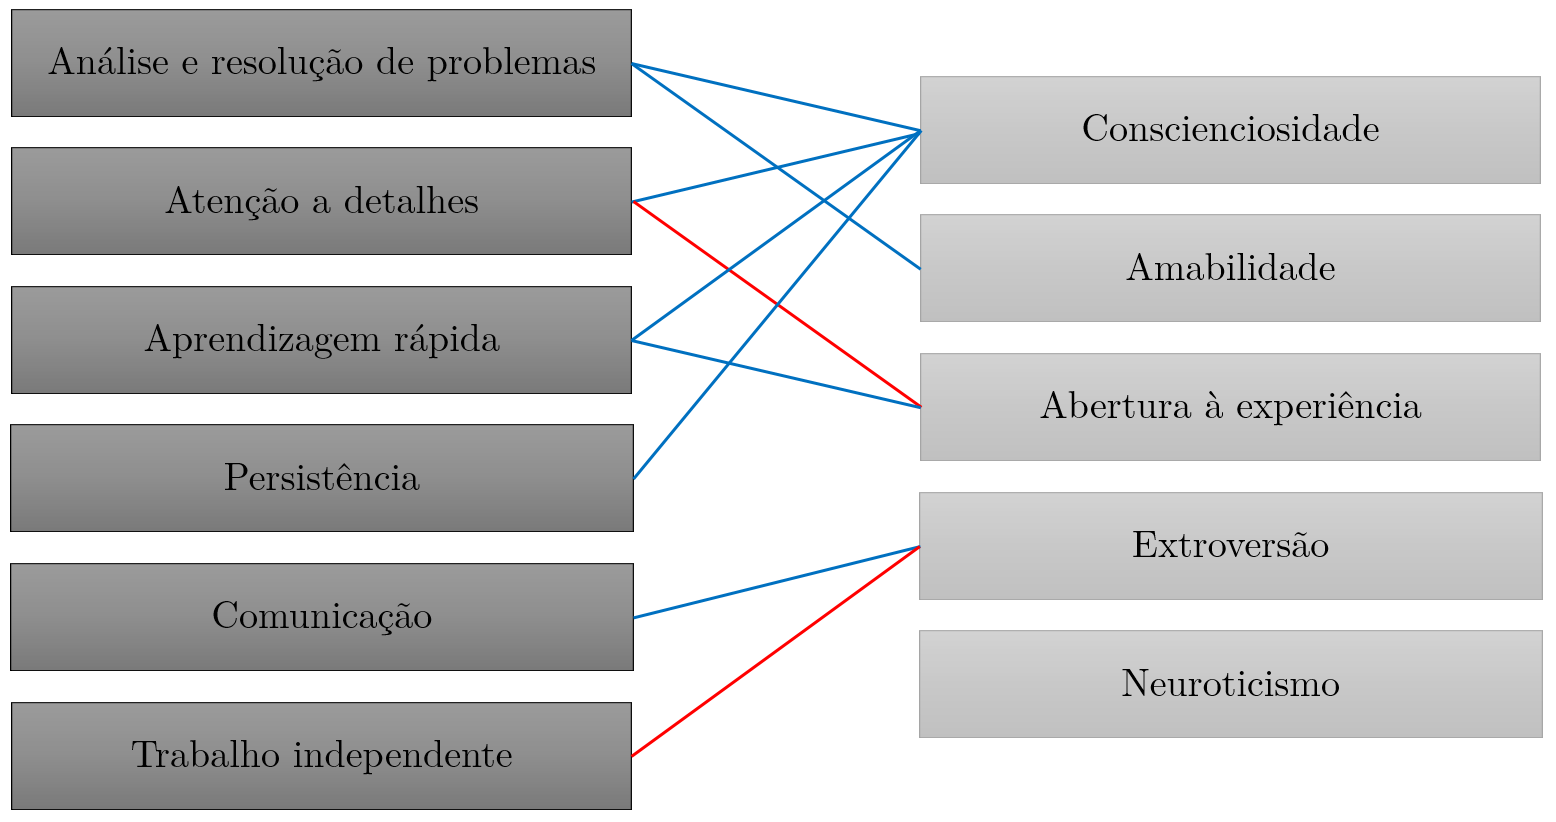
\includegraphics[width=.9\textwidth]{mapeamento.png}
\label{fig:mapeamento}
\end{figure}

Adicionalmente, na Figura \ref{fig:gerenciamento}, observamos a categorização das soft skills como estratégias para gerenciamento de tarefas, gerenciamento de si próprio, gerenciamento da carreira ou gerenciamento dos outros.

\begin{figure}[h*]
\centering
\caption{\small Categorização das soft skills como estratégias de gerenciamento} %\cite{litecky:04}} Precisa citar outra vez na imagem? 
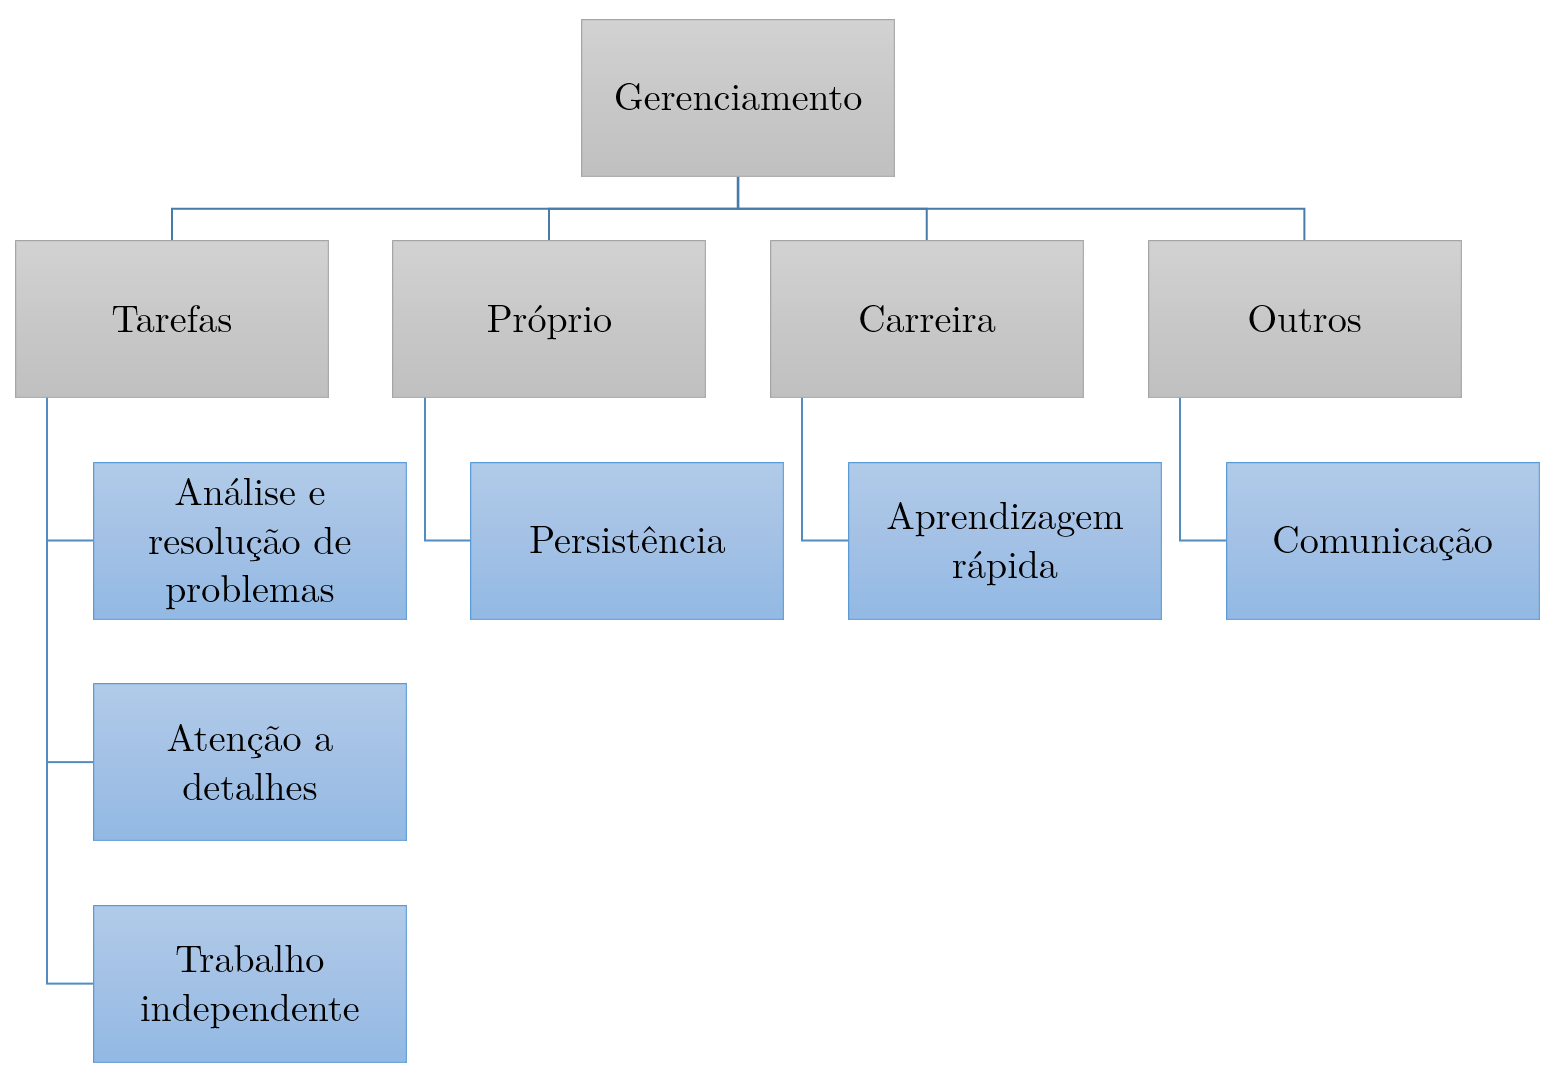
\includegraphics[width=.9\textwidth]{gerenciamento.png}
\label{fig:gerenciamento}
\end{figure}